% Options for packages loaded elsewhere
\PassOptionsToPackage{unicode}{hyperref}
\PassOptionsToPackage{hyphens}{url}
\PassOptionsToPackage{dvipsnames,svgnames,x11names}{xcolor}
%
\documentclass[
  12pt]{article}

\usepackage{amsmath,amssymb}
\usepackage{iftex}
\ifPDFTeX
  \usepackage[T1]{fontenc}
  \usepackage[utf8]{inputenc}
  \usepackage{textcomp} % provide euro and other symbols
\else % if luatex or xetex
  \usepackage{unicode-math}
  \defaultfontfeatures{Scale=MatchLowercase}
  \defaultfontfeatures[\rmfamily]{Ligatures=TeX,Scale=1}
\fi
\usepackage{lmodern}
\ifPDFTeX\else  
    % xetex/luatex font selection
\fi
% Use upquote if available, for straight quotes in verbatim environments
\IfFileExists{upquote.sty}{\usepackage{upquote}}{}
\IfFileExists{microtype.sty}{% use microtype if available
  \usepackage[]{microtype}
  \UseMicrotypeSet[protrusion]{basicmath} % disable protrusion for tt fonts
}{}
\makeatletter
\@ifundefined{KOMAClassName}{% if non-KOMA class
  \IfFileExists{parskip.sty}{%
    \usepackage{parskip}
  }{% else
    \setlength{\parindent}{0pt}
    \setlength{\parskip}{6pt plus 2pt minus 1pt}}
}{% if KOMA class
  \KOMAoptions{parskip=half}}
\makeatother
\usepackage{xcolor}
\setlength{\emergencystretch}{3em} % prevent overfull lines
\setcounter{secnumdepth}{5}
% Make \paragraph and \subparagraph free-standing
\ifx\paragraph\undefined\else
  \let\oldparagraph\paragraph
  \renewcommand{\paragraph}[1]{\oldparagraph{#1}\mbox{}}
\fi
\ifx\subparagraph\undefined\else
  \let\oldsubparagraph\subparagraph
  \renewcommand{\subparagraph}[1]{\oldsubparagraph{#1}\mbox{}}
\fi


\providecommand{\tightlist}{%
  \setlength{\itemsep}{0pt}\setlength{\parskip}{0pt}}\usepackage{longtable,booktabs,array}
\usepackage{calc} % for calculating minipage widths
% Correct order of tables after \paragraph or \subparagraph
\usepackage{etoolbox}
\makeatletter
\patchcmd\longtable{\par}{\if@noskipsec\mbox{}\fi\par}{}{}
\makeatother
% Allow footnotes in longtable head/foot
\IfFileExists{footnotehyper.sty}{\usepackage{footnotehyper}}{\usepackage{footnote}}
\makesavenoteenv{longtable}
\usepackage{graphicx}
\makeatletter
\def\maxwidth{\ifdim\Gin@nat@width>\linewidth\linewidth\else\Gin@nat@width\fi}
\def\maxheight{\ifdim\Gin@nat@height>\textheight\textheight\else\Gin@nat@height\fi}
\makeatother
% Scale images if necessary, so that they will not overflow the page
% margins by default, and it is still possible to overwrite the defaults
% using explicit options in \includegraphics[width, height, ...]{}
\setkeys{Gin}{width=\maxwidth,height=\maxheight,keepaspectratio}
% Set default figure placement to htbp
\makeatletter
\def\fps@figure{htbp}
\makeatother

\addtolength{\oddsidemargin}{-.5in}%
\addtolength{\evensidemargin}{-1in}%
\addtolength{\textwidth}{1in}%
\addtolength{\textheight}{1.7in}%
\addtolength{\topmargin}{-1in}%

\usepackage{amsthm}
\newtheorem{ass}{Assumption}
% \usepackage{mathtools}
\usepackage[final, nomargin, inline, nomarginclue, author=HM]{fixme}
% \fxusetargetlayout{color}
\fxsetface{inline}{\color{blue}}
\fxsetface{env}{\color{blue}}
% \usepackage{amsmath}
% \usepackage[final,nomargin,index,inline, author=]{fixme}
% \usepackage{bbm}
\usepackage{unicode-math}
\usepackage{tabularx}
\usepackage{adjustbox}
% \usepackage{amsmath}
% - \usepackage{longtable}
% - \usepackage{booktabs}
% - \usepackage{graphicx}
% \newtheorem{definition}{Definition}
% \newtheorem{theo}{Theorem}
% \newtheorem{lemma}{Lemma}
% \newtheorem{ass}{Assumption}
% \usepackage{xkvltxp}
% -  #final or draft
% - \fxsetup{envlayout=color, targetlayout=color}
% - \fxsetface{inline}{\color{blue}}

% kableExtra required packages:
\usepackage{booktabs}
\usepackage{longtable}
% \usepackage{array}
% \usepackage{multirow}
% \usepackage{wrapfig}
% \usepackage{float}
% \usepackage{colortbl}
% \usepackage{pdflscape}
% \usepackage{tabu}
\usepackage{threeparttable}
\usepackage{threeparttablex}
% \usepackage[normalem]{ulem}
% \usepackage{makecell}
% \usepackage{xcolor}
\usepackage{booktabs}
\usepackage{longtable}
\usepackage{array}
\usepackage{multirow}
\usepackage{wrapfig}
\usepackage{float}
\usepackage{colortbl}
\usepackage{pdflscape}
\usepackage{tabu}
\usepackage{threeparttable}
\usepackage{threeparttablex}
\usepackage[normalem]{ulem}
\usepackage{makecell}
\usepackage{xcolor}
\usepackage{tabularray}
\usepackage[normalem]{ulem}
\usepackage{graphicx}
\UseTblrLibrary{booktabs}
\UseTblrLibrary{siunitx}
\NewTableCommand{\tinytableDefineColor}[3]{\definecolor{#1}{#2}{#3}}
\newcommand{\tinytableTabularrayUnderline}[1]{\underline{#1}}
\newcommand{\tinytableTabularrayStrikeout}[1]{\sout{#1}}
\makeatletter
\@ifpackageloaded{caption}{}{\usepackage{caption}}
\AtBeginDocument{%
\ifdefined\contentsname
  \renewcommand*\contentsname{Table of contents}
\else
  \newcommand\contentsname{Table of contents}
\fi
\ifdefined\listfigurename
  \renewcommand*\listfigurename{List of Figures}
\else
  \newcommand\listfigurename{List of Figures}
\fi
\ifdefined\listtablename
  \renewcommand*\listtablename{List of Tables}
\else
  \newcommand\listtablename{List of Tables}
\fi
\ifdefined\figurename
  \renewcommand*\figurename{Figure}
\else
  \newcommand\figurename{Figure}
\fi
\ifdefined\tablename
  \renewcommand*\tablename{Table}
\else
  \newcommand\tablename{Table}
\fi
}
\@ifpackageloaded{float}{}{\usepackage{float}}
\floatstyle{ruled}
\@ifundefined{c@chapter}{\newfloat{codelisting}{h}{lop}}{\newfloat{codelisting}{h}{lop}[chapter]}
\floatname{codelisting}{Listing}
\newcommand*\listoflistings{\listof{codelisting}{List of Listings}}
\usepackage{amsthm}
\theoremstyle{definition}
\newtheorem{definition}{Definition}[section]
\theoremstyle{remark}
\AtBeginDocument{\renewcommand*{\proofname}{Proof}}
\newtheorem*{remark}{Remark}
\newtheorem*{solution}{Solution}
\newtheorem{refremark}{Remark}[section]
\newtheorem{refsolution}{Solution}[section]
\makeatother
\makeatletter
\makeatother
\makeatletter
\@ifpackageloaded{caption}{}{\usepackage{caption}}
\@ifpackageloaded{subcaption}{}{\usepackage{subcaption}}
\makeatother
\makeatletter
\@ifpackageloaded{tcolorbox}{}{\usepackage[many]{tcolorbox}}
\makeatother
%%%% ---foldboxy preamble ----- %%%%%

\definecolor{fbx-default-color1}{HTML}{c7c7d0}
\definecolor{fbx-default-color2}{HTML}{a3a3aa}

\definecolor{fbox-color1}{HTML}{c7c7d0}
\definecolor{fbox-color2}{HTML}{a3a3aa}

% arguments: #1 typelabelnummer: #2 titel: #3
\newenvironment{fbx}[3]{\begin{tcolorbox}[enhanced, breakable,%
attach boxed title to top*={xshift=1.4pt},
boxed title style={boxrule=0.0mm, fuzzy shadow={1pt}{-1pt}{0mm}{0.1mm}{gray}, arc=.3em, rounded corners=east, sharp corners=west}, colframe=#1-color2, colbacktitle=#1-color1, colback = white, coltitle=black,  titlerule=0mm, toprule=0pt, bottomrule=.7pt, leftrule=.3em, rightrule=0pt, outer arc=.3em,  arc=0pt,	 sharp corners = east, left=.5em, bottomtitle=1mm, toptitle=1mm,title=\textbf{#2}\hspace{0.5em}{#3}]}
{\end{tcolorbox}}

% boxed environment with right border
\newenvironment{fbxSimple}[3]{\begin{tcolorbox}[enhanced, breakable,%
attach boxed title to top*={xshift=1.4pt},
boxed title style={boxrule=0.0mm, fuzzy shadow={1pt}{-1pt}{0mm}{0.1mm}{gray}, arc=.3em, rounded corners=east, sharp corners=west}, colframe=#1-color2, colbacktitle=#1-color1, colback = white, coltitle=black,  titlerule=0mm, toprule=0pt, bottomrule=.7pt, leftrule=.3em, rightrule=.7pt, outer arc=.3em,  	left=.5em, right=.5em, bottomtitle=1mm, toptitle=1mm,title=\textbf{#2}\hspace{0.5em}{#3}]}
{\end{tcolorbox}}

%%%% --- end foldboxy preamble ----- %%%%%
%%==== colors from yaml ===%
\definecolor{Proposition-color1}{HTML}{99CCFF}
\definecolor{Proposition-color2}{HTML}{FFFFFF}
\definecolor{Assumption-color1}{HTML}{99CCFF}
\definecolor{Assumption-color2}{HTML}{FFFFFF}
\definecolor{Definition-color1}{HTML}{99CCFF}
\definecolor{Definition-color2}{HTML}{FFFFFF}
\definecolor{Theorem-color1}{HTML}{99CCFF}
\definecolor{Theorem-color2}{HTML}{FFFFFF}
%=============%
\ifLuaTeX
  \usepackage{selnolig}  % disable illegal ligatures
\fi
\usepackage[]{natbib}
\bibliographystyle{agsm}
\usepackage{bookmark}

\IfFileExists{xurl.sty}{\usepackage{xurl}}{} % add URL line breaks if available
\urlstyle{same} % disable monospaced font for URLs
\hypersetup{
  pdftitle={Tax Evasion and Productivity},
  pdfauthor={Hans Martinez},
  pdfkeywords={Tax Evasion, Cost Overreporting, Production Function
Estimation, Productivity},
  colorlinks=true,
  linkcolor={blue},
  filecolor={Maroon},
  citecolor={Blue},
  urlcolor={Blue},
  pdfcreator={LaTeX via pandoc}}


\begin{document}


\def\spacingset#1{\renewcommand{\baselinestretch}%
{#1}\small\normalsize} \spacingset{1}


%%%%%%%%%%%%%%%%%%%%%%%%%%%%%%%%%%%%%%%%%%%%%%%%%%%%%%%%%%%%%%%%%%%%%%%%%%%%%%

\date{April 13, 2024}
\title{\bf Tax Evasion and Productivity}
\author{
Hans Martinez\thanks{email: hmarti33@uwo.ca. I thank my supervisors
Salvador Navarro, David Rivers, and Victor Aguiar for their guidance.}\\
Department of Economics, University of Western Ontario\\
}
\maketitle

\bigskip
\bigskip
\begin{abstract}
Corporate tax evasion through cost overreporting spreads internationally
causing governments significant tax revenue losses. Detecting and
measuring the magnitude of tax evasion remains a challenge, even for the
few studies on overreporting where researchers can exploit
administrative data. Moreover, if this evasion strategy accounts for
economic losses as large as reported, then cost overreporting might bias
estimates of production functions, especially productivity. This paper
addresses both issues. I first provide a novel strategy to estimate cost
overreporting using commonly available firm-level data. I then formally
show that ignoring cost overreporting leads to downward biased
productivity estimates. Finally, I demonstrate how to recover
productivity in the presence of tax evasion.
\end{abstract}

\noindent%
{\it Keywords:} Tax Evasion, Cost Overreporting, Production Function
Estimation, Productivity
\vfill

\newpage
\spacingset{1.9} % DON'T change the spacing!

\section*{Introduction}\label{introduction}
\addcontentsline{toc}{section}{Introduction}

Corporate tax evasion through cost overreporting spreads globally
causing governments significant tax revenue losses. Detecting and
measuring the magnitude of cost overreporting remains a challenge, even
for researchers with access to government administrative data. Moreover,
if this evasion strategy accounts for economic losses as large as
reported, then cost overreporting might bias estimates of production
functions, including productivity. This paper addresses both issues. I
first provide a novel strategy to estimate cost overreporting using more
commonly available firm-level data. I then formally show that ignoring
cost overreporting leads to downward biased productivity estimates.
Finally, I demonstrate how to recover unbiased estimates of the
production function and productivity in the presence of tax evasion.

Cost overreporting arises when firms acquire false invoices to claim
additional tax deductions on value-added (VAT) and corporate income
taxes (CIT). According to the OECD's document \citet{OECD2017}, cost
overreporting --- also known as ``fake invoicing'', ``ghost firms'',
``invoice mills'', or ``missing traders''--- permeates internationally.
Reports from Latin America, Eastern Europe, Asia, and Africa claim cost
overreporting led to annual tax revenue losses as large as 5.6\% of the
GDP, for example, in Poland, 2016 (Poland's Minister of Finance,
2018)\footnote{Other reports show that cost overreporting led to revenue
  losses of 0.2\% of Chile's GDP in 2004 (Gonzalez and Velasquez, 2013;
  Jorrat, 2001; CIAT, 2008); 0.2\% of Colombia's GDP (Portafolio, 2019);
  and 0.03\% of Mexico's GDP in 2018 (Senado de la Republica, 2019).}
\fxnote{how does it compare to other forms of tax evasion?}

Despite its relevance, cost overreporting has been mostly overlooked by
the literature. On one hand, the few studies on this evasion strategy
exploit detailed administrative data \citep{Zumaya2021, Carrillo2022}.
Government tax authorities restrict access to administrative data
because of firms' confidentiality concerns. On the other hand, to the
best of my knowledge, no study has attempted to structurally identify
cost overreporting. Unlike the case of individuals
\citep{Pissarides1989, Paulus2015}, when it comes to corporate tax
evasion, researchers have to account for an additional source of
unobserved heterogeneity, productivity. Why? Because cost overreporting
might be naively quantified as low productivity. Intuitively, for a
given output level, high input utilization by a firm could be explained
by either the amount of input the firm overreports to evade taxes or by
a negative productivity shock.

To address this gap in the literature, first I formally show that
ignoring tax evasion leads to downwardly biased productivity estimates.
I then provide a new estimation strategy, requiring only commonly
available firm-level data, to jointly recover the densities of tax
evasion and productivity. The intuition works as follows. In the absence
of tax evasion, the first-order conditions of the firms'
cost-minimization problem inform about a common technology, the
production function. Consequently, in the presence of cost
overreporting, deviations from this common technology identify tax
evasion up to the current-period output shock. Then, from the subset of
non-overreporting firms, the strategy identifies the production function
parameters and the density of the output shock. Finally, using
deconvolution techniques, I can jointly recover the distributions of tax
evasion and productivity. \fxnote{I also estimate how tax evasion
evolves with productivity, in other words, their joint distribution}

I am currently working on an application of the method using firm-level
data from Colombia between 1981 and 1991. Colombia is an interesting
case because two major fiscal reforms in this period will allow me to
show how to apply the method to evaluate a policy change. I include a
description of the Colombian Tax System of the time. The plan is to also
have estimates for Ecuador and Mexico. Both of these countries have
administrative data which I plan to use to evaluate the method's
estimates.

\begin{anfxnote}{Remove}
Recently, evidence from Ecuador \citep{Carrillo2022} shows that cost
overreporting disseminates across all types of firms; constitutes a
quantitatively large share of firms' total deductions; and occurs mostly
in the intermediate inputs. Contrary to the literature consensus,
evasion by overreporting is not limited to small, semi-formal firms, but
large and formal firms overreport too. Likewise, firms were found to
overreport up to 14.1\% of the value of their purchase deductions.
Finally, when challenged by the tax authority, firms adjusted mostly
intermediate inputs.

The evidence from Ecuador also shows that big firms do not overreport
inputs. This is unsurprising for several reasons. First, a large firm
arguably draws more attention from the tax authority. Given its limited
resources, the government optimizes its expected revenues by targeting
the firms with the higher potential tax recovery, the few big ones.
Second, the cost of being caught cheating is potentially higher for big
firms. Large firms are likely to participate in international markets. A
tax evasion scandal in Colombia, for example, might affect US sales.
Finally, big firms potentially have more sophisticated strategies for
tax evasion \citep[e.g., profit shifting][]{Bustos2022}.

In a preliminary application, I show how to use the method to learn
about tax evasion even when we do not know the subset of non-evading
firms, but there has been a change in fiscal policy that incentivizes
cost overreporting. Using firm-level data from Colombia between 1981 and
1991, I show that tax evasion through cost overreporting increased after
the fiscal reform of 1983 between 8 and 9\% in 1985 and 1986. This
result stands at odds with previous studies that indicate that the
evasion of income tax and VAT declined during this period (Sanchez \&
Gutierrez, 1994)

I formally show that ignoring tax evasion leads to biased estimates of
productivity, which can be significant considering cost overreporting is
widespread and quantitatively large. In the proxy variable literature,
productivity is measured as the residual of a production function, where
the output is a function of the inputs. A key assumption is that input
demand is strictly monotonic on the productivity
\citep{Gandhi2020, Ackerberg2015, Levinsohn2003}. In other words, we
expect highly productive firms will use fewer inputs and produce more
output. When firms overreport their costs (inputs) to reduce their tax
liabilities, their reported inputs are higher than their actual
utilization, resulting in lower productivity estimates.

Tax evasion through cost overreporting has been largely overlooked by
the literature, though; most recent studies focus on revenue
underreporting.

Despite its relevance, detecting and measuring tax evasion ---through
cost overreporting or otherwise--- remains a non-trivial task even for
governments with detailed administrative data; mainly because of firms'
---and individuals'--- incentives to avoid getting caught. Direct
empirical measures are mostly unreliable because firms and individuals
have incentives to conceal their behavior \citep{Slemrod2019}. Hence, it
is unlikely that evasion would be truthfully reported in surveys, for
instance. Indirect structural measures have had some degree of success
in the case of individual income tax evasion \citep{Pissarides1989}, but
in the case of corporate tax evasion researchers must account for an
additional latent variable, the productivity of firms. The reason is
that tax evasion might be naively quantified as low productivity.
Intuitively, for a given level of output, high input utilization by a
firm could be explained by either the amount of input the firm
overreports to evade taxes or by a low productivity shock. In certain
countries, governments take advantage of the different sources of
administrative data. For example, in Ecuador, the tax authority uses
third-party information on reported corporate taxes to detect evasion
through revenue underreporting \citep{Carrillo2017}. However, access to
this type of administrative data is generally restricted for most
researchers.

Despite the vast efforts of the literature, measuring tax evasion
remains a non-trivial task\footnote{The challenge is to obtain reliable
  data. Practitioners usually have to undergo time- and
  resource-consuming processes to access or collect data; for example,
  by requesting access to government administrative data or by
  collecting their own through surveys or experiments.}.

Tax evasion is a significant concern for developing and developed
countries\footnote{Tax evasion has been a long-standing concern for
  developing countries, but since the 2008 economic crisis, it has also
  been of increasing importance for developed countries
  \citep{Slemrod2019}.}.

Having productivity estimates could potentially help, however, tax
evasion has not been satisfactorily addressed in the estimation of
productivity. I show that ignoring tax evasion leads to biased estimates
of productivity. To address this gap in the literature, I provide a new
estimation strategy to recover tax evasion and productivity using
commonly available data.

Indirect structural attempts to estimate corporate tax evasion have to
account for the productivity of the firms. The reason is that low
productivity might be naively quantified as tax evasion. Consider the
case in which firms overreport input expenses to reduce their profits to
evade taxes. A practitioner with output and input data might conclude
that output is a function of inputs, thus it can be considered a second
measure. She might try to recover true inputs and get an estimate of tax
evasion by the difference between reported and true inputs. However, for
a given level of output, high input utilization by a firm could be
explained by either the amount of input the firm overreports to evade
taxes or by its low productivity.

Firm-level estimates of productivity could be helpful to measure tax
evasion, however, tax evasion has not been satisfactorily addressed in
the estimation of productivity by the literature. The literature has
coped with tax evasion by treating it as a classical measurement error
\citep[e.g.,][p.204]{Blalock2004}. In other words, it has been assumed
that tax-evasion misreporting has zero mean ---some firms under-report
and others over-report so that the misreporting does not bias the
estimates of interest--- and this misreporting is independent of
everything else, including the attributes of the firms. However, the
classical measurement error argument is inconsistent with economic
intuition\footnote{Economic intuition will inform us that systematic
  misreporting due to tax evasion should lead firms to decrease profits
  by either underreporting sales or overreporting costs. Put
  differently, there's no economic incentive for firms to go the other
  direction ---overreporting sales or underreporting input expenses---
  and artificially increase their profits. An artificial increment of
  profits will increase the tax liabilities of the firm and decrease
  their after-tax real profits. Therefore, it is unlikely that tax
  evasion is mean zero. Economic intuition will also point out that the
  degree of misreporting is likely to vary across firms depending on the
  characteristics of the firms, e.g., age, size, owner's risk aversion,
  etc.}.

The contribution to the tax evasion literature is two-fold: (1) I
provide an estimation strategy using commonly available data, and (2)
the method identifies tax evasion through cost overreporting, an
overlooked by the literature but relevant phenomenon. The contribution
to the productivity literature is to show that ignoring tax evasion
leads to biased estimates and to provide a method to recover the
productivity density in the presence of input overreporting.

Why do we care about productivity measurement bias due to tax evasion?
First, it might help explain part of the productivity gap puzzle.
Economists have found \emph{enormous and consistent} productivity
differences across producers \citep{Syverson2011}. We still don't know
how much of this productivity gap ---the difference between the lower
and higher percentiles of the distribution--- tax evasion can explain.
Second, it should be considered in the design of public policies aiming
at reducing resource misallocations. Aggregate productivity ---and,
thus, the economic growth of a country and the welfare of its
citizens--- depends on the efficient allocation of its inputs among its
firms. Ideally, resources should be allocated to the most productive
firms. Additionally, it is not necessarily the case that firms with the
highest incentives to evade taxes are always the lowest productive. The
incentives depend on the tax system. For example, in countries where a
profit threshold determines different tax rates, the firms near the
threshold are the ones with the highest incentives to misreport, but the
threshold might be completely unrelated to productivity. Therefore,
firm-level productivity estimates adjusted by tax evasion misreporting
might inform better the design of public policies aiming at an efficient
reallocation of resources to boost economic growth.

Moreover, accounting for tax evasion in estimating and measuring
firm-level productivity is particularly significant for developing
countries. This is the case because tax evasion is likely to be higher
in low- and middle-income countries\footnote{Informality ---the extreme
  form of tax evasion--- is larger in developing countries
  \citep{Loayza2006, LaPorta2014}.}, and because the productivity gap in
these countries is wider ---wider productivity gaps are associated with
higher resource misallocations. For example, recent estimates of
non-detected tax evasion are up to \$10 billion USD per year in Mexico
\citep{Zumaya2021}, approximately 1\% of the country's GDP. Furthermore,
some studies argue that input misallocation ---implied by a wider
productivity gap--- explains a significant part of the differences in
income per capita between developed and developing countries
\citep{Syverson2011, Levy2018}. For instance, evidence from Colombia
suggests that labor and financial policy reforms during the 1990s aimed
at reallocating away from low- and towards high-productivity firms
---effectively reducing the productivity gap--- resulted in a higher
aggregate productivity \citep{Eslava2004}.

The main challenge of dealing with tax evasion is that it is hidden by
nature, for that reason,

So, then, in this paper, I ask,

\begin{quote}
can we recover unbiased productivity estimates at the firm level using a
gross-output production function in the presence of systematic
misreporting due to tax evasion? if so, what is the magnitude of this
bias, in particular for developing countries? given that different tax
systems ---rates, rules and enforcement procedures--- generate different
tax evasion incentives, how does the producitivity bias vary according
to different tax systems? how much of the productivity gap can tax
evasion explain within a country and across countries?
\end{quote}

To answer these questions, this paper studies productivity at the
establishment level for Mexican and Colombian firms accounting for tax
evasion. I employ data from a sample of anonymized firms' tax filings
and INEGI's EAIM annual production survey, in the case of Mexico. For
Colombia, I use the EAM annual survey on manufacturing firms. In the
estimation framework, I jointly model the firm-level productivity and
the tax evasion, allowing for classical measurement error. The key
identifying assumption is that while tax evasion depends on the expected
return to cheating, productivity follows a Markov process, and
measurement error is uncorrelated with inputs and across time. In turn,
the expected returns to cheating depend on the firm's
characteristics\footnote{Tax evasion might also depend on the firm's
  market characteristics, e.g., market concentration, end-consumer
  vs.~intermediate goods market, etc.}. In particular, larger firms are
less likely to underreport inputs because of their higher cheating cost,
their higher probability to be anonymously denounced by an employee, and
their access to complex tools to legally \emph{avoid} taxes\footnote{I
  follow the literature by referring to evasion as illegal actions to
  reduce tax liability, while avoidance refers to legal actions to
  reduce tax.}.

By jointly modeling tax evasion and productivity, this paper departs
from the literature in estimating a latent variable that follows an
incentive constraint (IC) ---tax compliance---, and in focusing on the
productivity bias ---rather than on an input's coefficient. Recent work
has studied the effect of measurement error in capital inputs on
production function estimation. Their approach has been using an IV
\citep{Collard2020} or a centering condition \emph{à la} \citet{Hu2008}
(Charlotte's JMP). However, systematic misreporting is different from
measurement error in that it goes only one way and it follows an IC, as
discussed above. Likewise, because capital is not a flexible
input\footnote{In the literature, a flexible input is neither dynamic
  ---current input choice depends on its lagged value---, nor
  predetermined ---completely defined in the past.}, the focus of these
papers is on the effect of the marginal return to capital coefficient
rather than on the effect on productivity estimates.

Moreover, I focus on gross-output production functions, as opposed to
value-added, to reduce the noise that might be introduced by firms
cheating also on prices. Besides the fact that prices are an equilibrium
object and might be affected by demand also ---and not only by
supply---, firms might also artificially increase the price of inputs or
reduce the price of sales to reduce declared profits. Then, in that
sense, the tax-evasion bias magnitude of productivity estimates obtained
through a value-added production function would be greater than through
the gross-output production function. In the latter, only the price of
the flexible input ---intermediates---, and the output sale price enter
through the first-order conditions (FOC) of the profit maximization
problem of the firm\footnote{If the cross-derivative of the flexible
  input with respect to the non-flexible inputs is not zero, then
  systematic misreporting in the non-flexible inputs will also affect
  productivity.}. In contrast, the prices of the non-flexible inputs,
---capital and labor---, might introduce noise in the case of the
value-added production function.
\fxnote{tax evasion underreporting sales: use firms that sell to other firms because of opposite incentives in contrast to firm-end consumer sales. Unskilled labor might be flexible but it's the least productive, so less damage.}

\end{anfxnote}

\section{A parsimonious model of tax evasion through input
overreporting}\label{a-parsimonious-model-of-tax-evasion-through-input-overreporting}

Price-taking firms maximize expected after-tax profits. Firms choose the
flexible input \(M_{it}\) to produce output \(Y_{it}\) given output and
input prices \(\{P_{t}, \rho_t\}\), a common technology, the production
function (Equation~\ref{eq-prod-fn}), and their productivity
\(\omega_{it}\).

\begin{equation}\phantomsection\label{eq-prod-fn}{
Y_{it}=G(M_{it})\exp(\omega_{it}+\varepsilon_{it})
}\end{equation}

As standard in the literature, productivity \(\omega_{it}\) is known to
firms when they take input decisions. This is the well-known endogeneity
problem of simultaneity. On the other hand, firms face output shocks.
The output shock \(\varepsilon_{it}\) is not part of the firms'
information set.

The model departs from the literature by allowing firms to overreport
their inputs \(e_{it}\) to reduce their tax burden and optimize
after-tax profits. Firms, then, consider in their optimization problem
the profit tax \(\tau\), the evasion penalty/cost \(\kappa(e)\), and the
probability of detection \(q(e_{it}|\theta_{it})\).

Firms solve Equation~\ref{eq-eva}
\begin{equation}\phantomsection\label{eq-eva}{
\begin{aligned}
  \max_{M_{it}, e_{it}\in [0,\infty), } [1-q(e_{it}|\theta_{it})]&\left[(P_t\mathbb{E}[Y_{it}]-\rho_{t} M_{it})-\tau\left(P_t\mathbb{E}[Y_{it}]-\rho_{t} (M_{it}+e_{it})\right)\right]\\
  +q(e_{it}|\theta_{it})&\left[(1-\tau)(P_t\mathbb{E}[Y_{it}]-\rho_{t} M_{it})-\kappa(e)\right] \\
  \text{s.t. }\; Y_{it}=G(M_{it})\exp(\omega_{it}+\varepsilon_{it})
\end{aligned}
}\end{equation}

The probability of detection \(q(e_{it}|\theta_{it})\) is monotonically
increasing in the amount evaded \(e_{it}\), conditional on the type of
the firm \(\theta_{it}\). Intuitively, for a given type, firms that
evade more are more likely to get caught.

The type of the firm \(\theta_{it}\) might be discrete, like the type of
juridical organization, or continuous, like the level of
revenue\footnote{Level of revenue is a common measure for fiscal
  authorities to determine a firm's taxes and/or level of scrutiny,
  e.g., Mexico, Spain, Colombia, and Ecuador. \fxnote{Chile (?)}}. Some
types might be more likely to be detected if the firm engages in tax
evasion. For example, in contrast to other types of juridical
organizations in Colombia, corporations are closely supervised and are
required to have an auditor. That is, for a given level of tax evasion
\(e_0\) and two different types
\(\theta' \not= \theta \in \mathbfcal{\Theta}\), then
\(q(e_0|\theta')\ge q(e_0|\theta)\).

If the type \(\theta\) is continuous, it might be a function of inputs;
for example, level of revenue. Firms will then affect their probability
of detection \(q(e|\theta)\) in two ways: directly, by choosing how much
they evade \(e\); and indirectly, when choosing inputs \(M\).

The optimal decision of the firm will depend on the fiscal environment
\(\Gamma=\{\tau, \kappa, q \}\), namely the tax rates, the penalty/cost
of detection, and the probability of detection.

The firms' problem (Equation~\ref{eq-eva}) can be rewritten as follows,
\[
\begin{aligned}
  \max_{M_{it},e_{it}} \mathbb{E}[\pi_{it}|\Gamma] = &(1-\tau)\left(\mathbb{E}[Y_{it}]-\frac{\rho_{t}}{P_t} M_{it}\right)+[1-q(e_{it}|\theta_{it})]\left(\frac{\rho_{t}}{P_t}e_{it}\tau\right)
  -q(e_{it}|\theta_{it})\kappa(e_{it}) \\
  &\text{s.t. }\; Y_{it}=G(M_{it})\exp(\omega_{it}+\varepsilon_{it})
\end{aligned}
\]

Intuitively, if the firm overreports her inputs' cost, she will get the
share of the value she overreported with probability \((1-q)\) and she
will be penalized with probability \(q\).

Assuming well-behaved functions and no corner solutions, the first-order
conditions lead to the following system of differential equations,

\begin{equation}\phantomsection\label{eq-foc-cont-m}{
G_M(M_{it})\exp(\omega_{it})\mathcal{E}-\frac{\rho_{t}}{P_t} = \frac{1}{(1-\tau)}\frac{\partial q(e_{it}|\theta_{it})}{\partial \theta_{it}}\frac{\partial \theta_{it}}{\partial M}\left[\frac{\rho_t}{P_t}e_{it}\tau+\kappa(e_{it})\right]
}\end{equation}

\begin{equation}\phantomsection\label{eq-foc-cont-e}{
[1-q(e_{it}|\theta_{it})]\frac{\rho_t}{P_t}\tau-q(e_{it}|\theta_{it})\kappa'(e_{it})=q'(e_{it}|\theta_{it})\left[\frac{\rho_t}{P_t}\tau e_{it} + \kappa(e_{it})\right]
}\end{equation}

where \(\mathbfcal{E}=\mathbb{E}[\exp(\varepsilon_{it})]\). The type of
firms is continuous and increasing on the input. The probability of
detection is increasing in the type continuum. In particular,
\(\frac{\partial q(e_{it}|\theta_{it})}{\partial \theta_{it}}\frac{\partial \theta_{it}}{\partial M}\ge0\).

The left-hand side of Equation~\ref{eq-foc-cont-m} is the familiar
marginal output of inputs and the price ratio. In the absence of
incentives' distortions induced by the fiscal environment, they are
equal. But now, the equality holds no more. There's a wedge arising from
the fiscal environment. The right-hand side of the equation is positive
by the assumptions of the model.

Equation~\ref{eq-foc-cont-e} solves the optimal evasion decision. The
left-hand side is the marginal benefit net of the marginal cost of
evasion. The right-hand side is the rate of change of the probability of
detection due to a change in evasion weighted by the benefit and cost of
evading.

\subsection{\texorpdfstring{Case 1 (Independence): \(q(e|\theta)=q(e)\)
and
\(\kappa(e)=\kappa_0\)}{Case 1 (Independence): q(e\textbar\textbackslash theta)=q(e) and \textbackslash kappa(e)=\textbackslash kappa\_0}}\label{case-1-independence-qethetaqe-and-kappaekappa_0}

Consider the case when the probability of detection is independent of
type, \(q(e|\theta)=q(e)\). This could be the case if the type is the
juridical organization of the firm. Hence, the type of the firm, and
thus the probability of detection, does not change with the firm's input
decisions,
\(\frac{\partial q(e_{it}|\theta_{it})}{\partial \theta_{it}}\frac{\partial \theta_{it}}{\partial M}=0\).
In addition, assume the evasion cost is constant,
\(\kappa(e)=\kappa_0\), for simplicity.

In this case, the first-order conditions of Equation~\ref{eq-eva} with
respect to the input \(M_{it}\) and the tax evasion \(e_{it}\) yield the
following

\begin{equation}\phantomsection\label{eq-foc:ind}{
G_M(M_{it})\exp(\omega_{it})\mathcal{E}=\frac{\rho_{t}}{P_t}
}\end{equation}

\begin{equation}\phantomsection\label{eq-foc:eva:ind}{
e_{it}=\frac{1-q(e_{it})}{q'(e_{it})}-\frac{\kappa_0}{\frac{\rho_{t}}{P_t}\tau}
}\end{equation}

Equation~\ref{eq-foc:ind}, the well-known optimality condition, says
that the price ratio is equal to the marginal product of the inputs.

Likewise, Equation~\ref{eq-foc:eva:ind} reveals the firms' optimal tax
evasion decision decreases if the probability of detection \(q(e_{it})\)
or the penalty of evading \(\kappa\) increases. Tax evasion also depends
on how sensitive the probability of detection is to the level of evasion
\(q'(e)\). In particular, greater sensibility will result in lower
levels of evasion.

Note that the net change of tax evasion due to an increase in the
relative prices \(\frac{\rho_{t}}{P_t}\) or the tax rate \(\tau\) is not
evident at first sight. The net effect will also depend on the change in
the detection probability induced by the changes in the relative prices
or the tax rate. In particular, an increase in relative prices
\(\frac{\rho_{t}}{P_t}\) or the tax rate \(\tau\) will incentivize a
higher tax evasion level, however, a higher tax evasion level will
increase the probability of detection ---depending on the shape of the
probability as a function of \(e\)---, so it will deter higher levels of
evasion. An increase in the tax rate, for instance, will only increase
tax evasion if the change in the tax rates increases the incentives to
evade more than the decrease in the incentives due to the changes in the
detection probability.

Formally, suppose a firm increases its tax evasion, \(e_1-e_0>0\)
because of an increase in taxes \(\tau_1>\tau_0\). Then, it follows that

\[
\left(\frac{\tau_1-\tau_0}{\tau_1\tau_0}\right)\frac{P\kappa}{\rho}>
  \left(\frac{1-q(e_1)}{q'(e_1)}-\frac{1-q(e_0)}{q'(e_0)}\right)
\]

The change in the probability of detection weighted by the slope of the
probability function should be less than the change in the tax rate
weighted by the penalty of evading and the relative prices\footnote{An
  analogous condition for an increase in relative prices leading to
  higher levels of tax evasion exists. Under this condition, the model
  is consistent with the literature that macroeconomic downturns lead to
  higher evasion.}.

\subsection{Case 2 (Spain): Discrete increase in the probability of
detection after a certain threshold of
revenue}\label{case-2-spain-discrete-increase-in-the-probability-of-detection-after-a-certain-threshold-of-revenue}

In Spain, the Large Taxpayers Unit (LTU) of the tax authority focuses
exclusively on firms with total operating revenue above 6 million euros.
The LTU has more auditors per taxpayer than the rest of the tax
authority, and these auditors are on average more experienced and better
trained to deal with the most complex taxpayers. This LTU creates a
discontinuity in the monitoring effort of the tax authority.
Consequently, at this arbitrary revenue level, the probability of
detection increases discretely \citep{Almunia2018}.

In this scenario, depending on the productivity shock, the firm might be
better off choosing not to produce past the revenue threshold. Indeed,
for a relevant range of productivity draws
\(\Omega^B=[\omega^L, \omega^H]\), the firms will not choose to grow
past the revenue threshold if the expected after-tax profits of staying
small are greater than the expected after-tax profits of growing.

In the model, there is now a threshold of revenue \(\theta^L\) after
which the probability of detection increases discretely. To make things
simpler, assume that before the threshold, the probability changes as a
function of evasion but does not vary conditional on size. After the
threshold, the probability increases for every level of evasion but does
not vary conditional on size.

Formally, let \(\Theta_{L} = \{\theta_i : \theta_{i} < \theta^L \}\) and
\(\Theta_{H} = \{\theta_i : \theta_{i} \ge \theta^L \}\), then for all
\(e_0\) and \(\theta'_i\not=\theta_i\),
\(q(e_0|\theta_i \in \Theta_k)=q(e_0|\theta'_i \in \Theta_k)\) with
\(k=\{L,H\}\), but
\(q(e_0|\theta'_i \in \Theta_H)\ge q(e_0|\theta_i \in \Theta_L)\).

Firms' revenue with productivity draw \(\omega^L\) corresponds exactly
to the enforcement threshold \(\theta^L\). Production and reporting
decisions of firms with productivity draws below \(\omega^L\) are not
affected by the change in the probability of detection. Firms choose
their inputs according to Equation~\ref{eq-foc:ind} and their evasion
decision according to Equation~\ref{eq-foc-cont-e}. Firms with
productivity draws above \(\omega^U\)

Firms with productivity \(\omega_{i}\in \Omega^B\) will choose the input
level \(\tilde{M}_{i}\) resulting in an expected revenue below the
threshold \(\theta_{i}<\theta^L\), if the expected after-tax profit of
staying small are greater than growing,
\(\mathbb{E}[\pi_{i}|\Theta_L, \Omega^B]-\mathbb{E}[\pi_{i}|\Theta_H, \Omega^B]\ge0\).

The optimal input choice \(M^*_{i}\) for firms with productivity
\(\omega_i\in\Omega^B\) implies an expected revenue greater than or
equal to the threshold \(\theta^*_{i}\ge \theta^L\). Let the expected
profits given \(M^*_{i}\) and the optimal tax evasion in the range of
size \(\theta_l\), \(e^*_{it}\), is
\(\pi_l\equiv\mathbb{E}[\pi(M^*_{it}, e^*_{it})|\theta_l]\). Let
\(\tilde{M}_{it}\) be the input level such that the expected revenue is
below the threshold \(\tilde{s}_{it}<\theta^L\) and \(\tilde{e}_{it}\)
be the optimal tax evasion in the range of size \(\theta_s\). Let also
the expected profits of staying small are
\(\pi_s\equiv\mathbb{E}[\pi(\tilde{M}_{it},\tilde{e}_{it})|\theta_s]\).

In this second case, therefore, firms might optimally choose to remain
small if, for a low productivity shock, the expected profits of not
growing are greater than the expected profits of growing
\(\pi_l<\pi_s\). Firms choosing to remain small will lead to a bunching
below the threshold in the size distribution of firms.

Besides the higher levels of evasion before the threshold ---simply
because of the higher probability of detection---, we can also expect
bunching firms to evade more than their similar-sized peers. At
\(\tilde{M}_{it}\), the optimization condition of
Equation~\ref{eq-foc:ind} no longer holds, hence, the marginal product
of the input is now greater than the relative prices. Therefore,
according to Equation~\ref{eq-foc:eva:ind}, bunching firms would
compensate for their \emph{higher} costs by increasing overreporting.

\subsubsection{Discussion}\label{discussion}

What is new in this paper relative to the literature is that it focuses
on the production function framework using public data whereas
\citet{Almunia2018} and other papers use a bunching estimator with
government administrative data which is difficult to access. Second, the
paper focuses on input overreporting rather than on revenue
underreporting, which is the relevant margin of evasion for
manufacturing firms. More on this point in the revenue underreporting
section. Finally, in contrast to \citet{Almunia2018} where the authors
conclude that misreporting does not imply real losses in production but
only fictitious reduction of the real sales, firms might optimally forgo
higher revenue levels if the expected profits of staying small and evade
taxes by misreporting are greater than the expected profits of growing
and avoid misreporting.

\subsection{Case 3 (Colombia \& Mexico): Discrete increase in the tax
rate after a revenue
threshold}\label{case-3-colombia-mexico-discrete-increase-in-the-tax-rate-after-a-revenue-threshold}

\subsubsection{Colombia, Individual
Proprietorships}\label{colombia-individual-proprietorships}

In Colombia between 1981 and 1991, individual firm proprietors were
subject to the individual income tax schedule. Individuals had
incentives to not form juridical organizations to avoid double taxation.
The tax authority suffered from severe limitations and inefficiencies at
the time.

In this case, after the revenue threshold, the tax rate increases
discretely but the probability of detection does not. The jump in the
tax rate generates the incentive to increase evasion. However, a higher
level of evasion increases the cost of evading by increasing the
probability of detection. If the cost of an increased evasion outweighs
the benefits of growing past the revenue threshold, the firms would
bunch below the cutoff.

\subsubsection{Mexico, Irreversible Change in Tax Regime after a Revenue
Threshold}\label{mexico-irreversible-change-in-tax-regime-after-a-revenue-threshold}

In Mexico, firms with annual revenues below 2 million pesos are taxed
under the REPECO (\emph{Regime de Pequeños Contribuyentes}) regime of
small contributors at 2 percent of annual revenues, while firms above
that threshold are taxed under the general regime at 30 percent. Firms
must transition to the general regime if revenues increase beyond the
threshold. Once in the general regime, firms cannot revert to the REPECO
regime.

Firms' decision is now dynamic. Firms will maximize the sum of current
and future after-tax profits. The discrete jump in the tax rate will
lead to a bunching below the threshold. Moreover, the bunching will be
exacerbated because firms will choose to grow past the cutoff only if
the future productivity shocks allow the firm to continue to be
profitable.

\subsection{Case 4 (Colombia): Firms first choose type, input decisions
do not affect the probability of
detection}\label{case-4-colombia-firms-first-choose-type-input-decisions-do-not-affect-the-probability-of-detection}

In Colombia between 1981 and 1991, Corporations were closely supervised
by the Superintendent of Corporations and were required to have an
auditor. All other firms were subject to the regular monitoring efforts
of the tax authority, which suffered from severe limitations and
inefficiencies at the time.

In the model, firms first choose their type. Input decisions do not
affect the probability of detection. However, if the type is
\emph{Corporation} the probability of detection is higher than
\emph{Partnership}. Firms maximize the sum of their expected profits. In
their optimization problem, firms will consider the sum of expected
productivity shocks and their corresponding probability of detection.
High-productivity firms will self-select into \emph{Corporations}.

\begin{anfxnote}{Heterogeneity}

\subsection{Other Sources of
Heterogeneity}\label{other-sources-of-heterogeneity}

Currently, only productivity. But, it can also be

\begin{itemize}
\tightlist
\item
  Probability of detection might be a random function (idiosyncratic
  random shocks on the beliefs about being detected)
\item
  Cost of evasion (different technologies of evasion)
\end{itemize}

\end{anfxnote}

\section{The empirical framework}\label{the-empirical-framework}

Suppose we have access to panel data, where we observe output
\(Y_{it}\), intermediate inputs \(M_{it}\), capital \(K_{it}\), labor
\(L_{it}\), and output \(P_{t}\) and intermediate input prices
\(\rho_t\) for \(I\) firms over \(T\) periods. Then our set of
observations is
\(\mathcal O = \{Y_{it}, M_{it}, K_{it}, L_{it}, P_{t}, \rho_t\}_{i\in I, t \in T}\).
As is standard in the literature, firms are price-takers and the
intermediates are flexible.

The objects of interest are the production function (PF),
\(Y_{it}=G(M_{it}, K_{it}, L_{it})e^{\omega_{it}+\varepsilon^Y_{it}}\),
and productivity \(\omega_{it}\). \(\varepsilon^Y_{it}\) is the current
period output shock. We are also interested in the Markov process of
productivity, which we assume is AR(1),
\(\omega_{it}=h(\omega_{it-1})+\eta_{it}\), with
\(\mathbb{E}[\eta_{it}|\omega_{it-1}]=0\).

\subsection{Tax evasion and the productivity
bias}\label{tax-evasion-and-the-productivity-bias}

Firms overreport their true intermediate inputs \(M^*_{it}\) by
\(e^{\varepsilon^M_{it}}\) to evade taxes. Then, reported inputs are

\[
M_{it}=M^*_{it}e^{\varepsilon^M_{it}}   
\]

with \(\varepsilon_{it}^M\ge0\) and
\(\varepsilon_{it}^M\not\perp M^*_{it}\).

It is fairly easy to see that the productivity bias, the difference
between the naively estimated \(\tilde\omega_{it}\) and true
productivity \(\omega_{it}\) is as follows:

\[
 \mathbb{E}[\tilde\omega_{it}|\mathcal{I}_{it}]-
    \mathbb{E}[\omega_{it}|\mathcal{I}_{it}] \le
      \ln\mathbb{E}\left[
        \frac{G(M^*_{it}, K_{it}, L_{it})}{G(M^*_{it}e^{\varepsilon^M_{it}}, K_{it}, L_{it})}\Bigg|\mathcal{I}_{it}\right] \le 0
\]

Where \(\mathcal{I}\) stands for the information set of firm \(i\) in
time \(t\).

The previous result holds because of Jensen's inequality and because
\(G(\cdot)\) is monotonically increasing in its arguments.

\section{Colombia 1981-1991}\label{colombia-1981-1991}

\subsection{Colombian Corporate Tax
System}\label{colombian-corporate-tax-system}

The relevant corporate taxes for input overreporting in Colombia during
this period are the Corporate Income Tax (CIT) and the Sales Tax. The
Sales Tax gradually transformed into a kind of Value-Added Tax (VAT).
Also relevant for the CIT are the different juridical organizations that
exist in Colombia.

This period was characterized by high levels of overall tax evasion
\citep{Sanchez1994}. The fiscal rules had a system of penalties and
interest that encouraged false and delinquent returns
\citep{McLure1989}. The fiscal authority was characterized by having an
inefficient auditing system, being overburdened, and legal loopholes
\citep{Perry1990}.

\subsubsection{Juridical Organizations}\label{juridical-organizations}

In Colombia, there are five types of juridical organizations:
Corporations, Partnerships, Limited Liability Companies, and Individual
Proprietorships.

Corporations (\emph{sociedad anónima}) are the typical associations of
capital. They are the counterpart of the US corporation. The capital of
a corporation is provided by the shareholders (no less than 5) and is
divided into tradable shares of equal value. Shareholders' liability is
limited to the capital contributed. Corporations are subject to the
Superintendent of Corporations and are closely supervised, being
required to have an auditor.

Joint Stock Companies (\emph{sociedad en comandita por acciones})
comprises two or more managing partners who are jointly and severally
liable, and five or more limited partners whose liability is limited to
their respective contributions. Joint Stock Companies are taxed as
Corporations. Its shares are tradable, like the shares of Corporations.

Partnerships are associations of two or more persons. Partners are
jointly and severally liable for the partnership's operations.
Partnerships include general partnerships (\emph{sociedad colectiva}),
de Facto partnerships (\emph{sociedades de hecho}), and ordinary limited
partnerships (\emph{sociedad en comandita simple}).

A limited liability company (\emph{sociedad de responsabilidad
limitada}) is an association of two or more persons ---not exceeding 20
(Fiscal Survey) or 25 (1992 \emph{EAM} survey documents)---, whose
shares cannot be traded. The personal liability of the partners is
limited to the capital contributed. The Limited Liability Company is
quite important in Colombia (Fiscal Survey).

Finally, proprietorships are individuals (natural persons) who allocate
part of their assets to conduct commercial activities.

There are other juridical organizations in the data that will be
excluded from the final analysis. These organizations are non-profit,
like cooperatives and community enterprises, or state industrial
enterprises, the proceeds of which come from taxes, fees, or special
contributions.

\subsubsection{Corporate Income tax}\label{corporate-income-tax}

The juridical organizations were subject to different Corporate Income
Tax rates. Corporations were taxed at a fixed rate of 40\%, while
Partnerships and Limited Liability companies at 20\%. Individual
proprietors were subject to the graduated Individual Tax Schedule
consisting of 56 rates, ranging from 0.50 to 51 percent.

Corporations were taxed on their distributed dividends, while
partnerships and limited liability companies were taxed on their
profits, whether or not distributed. Owners of juridical organizations
were double taxed, at the firm and the individual level, whereas the
income of proprietorships was taxed only once, at the individual level.

Since 1974, individuals and juridical organizations, except for limited
liability companies, were subject to the minimum presumptive income.
Rent (income and profits) was presumed to be no less than 8 percent of
net wealth (assets less depreciation, real estate, livestock,
securities).

Certain industries like airlines, publishing, and reforestation sectors,
and various activities in selected regions (primarily ``frontier'' and
other less developed ones) had their income tax exempted, limited, or
reduced.

\begin{longtable}[]{@{}
  >{\centering\arraybackslash}p{(\columnwidth - 8\tabcolsep) * \real{0.3934}}
  >{\centering\arraybackslash}p{(\columnwidth - 8\tabcolsep) * \real{0.0820}}
  >{\centering\arraybackslash}p{(\columnwidth - 8\tabcolsep) * \real{0.1803}}
  >{\centering\arraybackslash}p{(\columnwidth - 8\tabcolsep) * \real{0.1475}}
  >{\centering\arraybackslash}p{(\columnwidth - 8\tabcolsep) * \real{0.1967}}@{}}
\caption{Juridical Organizations in Colombia (1980s), A
Summary}\label{tbl-jo-summary}\tabularnewline
\toprule\noalign{}
\begin{minipage}[b]{\linewidth}\centering
Organization
\end{minipage} & \begin{minipage}[b]{\linewidth}\centering
Corporate Income Tax
\end{minipage} & \begin{minipage}[b]{\linewidth}\centering
Liability
\end{minipage} & \begin{minipage}[b]{\linewidth}\centering
Capital
\end{minipage} & \begin{minipage}[b]{\linewidth}\centering
Owners
\end{minipage} \\
\midrule\noalign{}
\endfirsthead
\toprule\noalign{}
\begin{minipage}[b]{\linewidth}\centering
Organization
\end{minipage} & \begin{minipage}[b]{\linewidth}\centering
Corporate Income Tax
\end{minipage} & \begin{minipage}[b]{\linewidth}\centering
Liability
\end{minipage} & \begin{minipage}[b]{\linewidth}\centering
Capital
\end{minipage} & \begin{minipage}[b]{\linewidth}\centering
Owners
\end{minipage} \\
\midrule\noalign{}
\endhead
\bottomrule\noalign{}
\endlastfoot
Corporation & 40\% (on distributed dividends) & Limited to capital
participation & Tradable capital shares & \(N\ge5\) \\
Limited Co. & 20\% (on profits) & Limited to capital participation &
Non-tradable capital shares & \(2\le N \le 20 (25)\) \\
Partnership & 20\% (on profits) & Full & Not a capital association &
\(N\ge2\) \\
Proprietorship & Individual Income Tax & Full & Owner & \(N=1\) \\
\end{longtable}

\subsubsection{Sales taxes}\label{sales-taxes}

Sales taxes were originally targeted at the manufacturing sector on
finished goods and imports. Since 1974, manufacturers were allowed to
credit taxes paid on any purchase made by the firm, except the
acquisition of capital goods \citep{Perry1990}. The credits worked
through a system of refunds. Consequently, the tax became a kind of
value-added tax (VAT).

The basic rate was 15 percent. There was also a preferential rate of 6
percent for certain industries like clothing, footwear, and major inputs
used for building popular housing, and a rate of 35 percent for luxury
goods. Exports, foodstuff, drugs, and textbooks were excluded from the
beginning. Also excluded were inputs, transportation equipment,
agricultural machinery, and equipment.

\subsubsection{Discussion}\label{discussion-1}

From Colombia's tax system, we can conclude that corporations are the
least likely to evade taxes by misreporting because of at least three
reasons. One, the Superintendent of Corporations closely monitored
corporations by requiring them to have an auditor. In the model, this
implies that the probability of detection is higher for them. Second,
free tradable shares impose an incentive to be profitable because the
market value of the shares might be negatively affected otherwise. In
other words, if a corporation fakely reports lower profits, the value of
its shares would likely decrease scaring away shareholders and potential
investors. Joint stock companies have freely tradable shares too. Three,
corporations pay CIT on distributed dividends, not on profits as
Partnerships and LLCs did. Corporations have an additional margin
regarding the income tax they pay because they decide when to pay
dividends. This might generate other types of incentives that might be
influenced by the corporation's policy regarding their dividends and the
demands of their shareholders. On the other hand, Proprietorships and
LLCs are subject to the incentive to evade CIT by artificially reducing
their profits.

Moreover, Proprietorships, Partnerships, and Limited Companies had
incentives to overreport inputs to evade VAT and CIT. The incentives to
evade varied across industries because the sales tax rate differed
between industries. The incentives to evade also varied within industry
sectors because juridical organizations within an industry were subject
to different CIT rates. There were additional sources of variation
depending on the firm's location due to local exemptions and sales
composition (inputs to other firms, to consumers, to the foreign
market).

Lastly, Individual proprietorships were likely to bunch at the
individual income thresholds because they were subject to individual
income tax which was increasing by brackets.

\subsection{Fiscal Reforms}\label{fiscal-reforms}

During this period, Colombia went through three major fiscal reforms
(1983, 1986, 1990).

\subsubsection{1983}\label{section}

The 1983 reform tried to alleviate the double taxation by introducing a
tax credit of 10\% of dividends received for individuals.

In addition, Law 9 of 1983 instituted a measure of presumptive income
equal to 2 percent of gross receipts to supplement the measure based on
net wealth. This reform was aimed specifically at the commerce and
service sectors; the former was thought to evade the wealth-based
presumptive tax by systematically understating inventories. In addition,
it extended the presumptive income tax to limited liability companies.

In 1983, the value-added tax (VAT) was extended to the retail level,
with a \emph{simplified system} being made available to small retailers
to ease compliance costs and the administrative burden.

The 1983 reform relatively unified the value-added tax (VAT) rates by
combining previously taxed goods at 6\% and 15 percent into 10\%. The
number of the products and services that were levied expanded.

In 1984, VAT exemptions for agricultural machinery, transportation
equipment, and certain other goods were eliminated.

\subsubsection{1986}\label{section-1}

The 1986 reforms unified the taxation of corporations and limited
liability companies by taxing both at a rate of 30\%. The top tax rate
applied to individual income was reduced from 49 to 30\%.

Double taxation was eliminated. The reform exempted corporate dividends
and participation in profits of limited liability companies from tax at
the individual shareholder/owner level.

Lastly, the 1986 reform relocated the tax collection and reception of
tax reports to the banking system, among other things.

\subsubsection{1990}\label{section-2}

The 1990 reform increased the VAT from 10\% to 12\%.

In addition, the individual income obtained from the sale of shares
through the stock market was exempted from taxation. Income tax was
waived for investment funds, mutual funds, and securities, and the rates
for remittances and income for foreign investment were reduced. Tax
amnesties were granted, and the sanitation tax was reduced to encourage
the repatriation of capital.

\subsubsection{Discussion}\label{discussion-2}

Increases in the VAT would increase the incentives to evade. Decreases
in CIT would decrease them. Intuitively, we expect higher levels of tax
evasion if tax rates increase.

The CIT homogenization between Corporations and LLCs in 1986 would have
motivated LLCs to incorporate. Likewise, the elimination of double
taxation also in 1986 would have motivated proprietorships to become
LLCs, Corporations, or Partnerships.

On the other hand, reporting more information to the tax authority ---
like the banking system being responsible for the collection and
reception of tax reports in 1986--- would decrease tax evasion.

\subsection{Data}\label{data}

The Colombian data is a well-known firm-level panel data set that has
been used in the estimation of production functions and productivity
before. The Colombian dataset comes from the Annual Survey of
Manufacturing (EAM) and contains information about manufacturing firms
with more than 10 employees from 1981 to 1991.

Besides the information on output, intermediates, capital, and labor,
the dataset includes the type of juridical organization and the sales
taxes. Table~\ref{tbl-sum-stats} offers some summary statistics.

\begin{table}

\caption{\label{tbl-sum-stats}Summary Statistics, Manufacturing Firms in
Colombia (1981-1991)}

\centering{

\centering
\begin{tblr}[         %% tabularray outer open
]                     %% tabularray outer close
{                     %% tabularray inner open
colspec={Q[]Q[]Q[]Q[]Q[]Q[]},
hline{8}={1,2,3,4,5,6}{solid, 0.1em, black},
}                     %% tabularray inner close
\toprule
& Missing & Mean & SD & Min & Max \\ \midrule %% TinyTableHeader
Capital & 0 & 81450.0 & 1396998.4 & 1.0 & 270221640.5 \\
Materials \& Services & 0 & 144808.3 & 714091.1 & 13.0 & 35370843.8 \\
Labor (Skilled) & 0 & 30.1 & 82.9 & 1.0 & 7389.0 \\
Labor (Unskilled) & 0 & 67.0 & 149.2 & 1.0 & 5174.0 \\
Revenue & 0 & 219548.2 & 908964.3 & 82.2 & 44236868.0 \\
Sales Taxes & 0 & 13449.8 & 124432.7 & 0.0 & 16441078.0 \\
JO\_class & N & \% &  &  &  \\
Corporation & 8805 & 21.0 &  &  &  \\
Ltd. Co. & 25643 & 61.3 &  &  &  \\
Other & 541 & 1.3 &  &  &  \\
Partnership & 1462 & 3.5 &  &  &  \\
Proprietorship & 5380 & 12.9 &  &  &  \\
\bottomrule
\end{tblr}

}

\end{table}%

A simple graphical analysis shows that the average (of the log)
intermediates cost share of sales started growing after 1983 and that it
stabilized in 1988 after the policy changes of the 1986 reform settled
in (Figure~\ref{fig-logshare}). The dataset does not capture any changes
after the 1990 reform, although there is only one more year of data.

\begin{figure}

\centering{

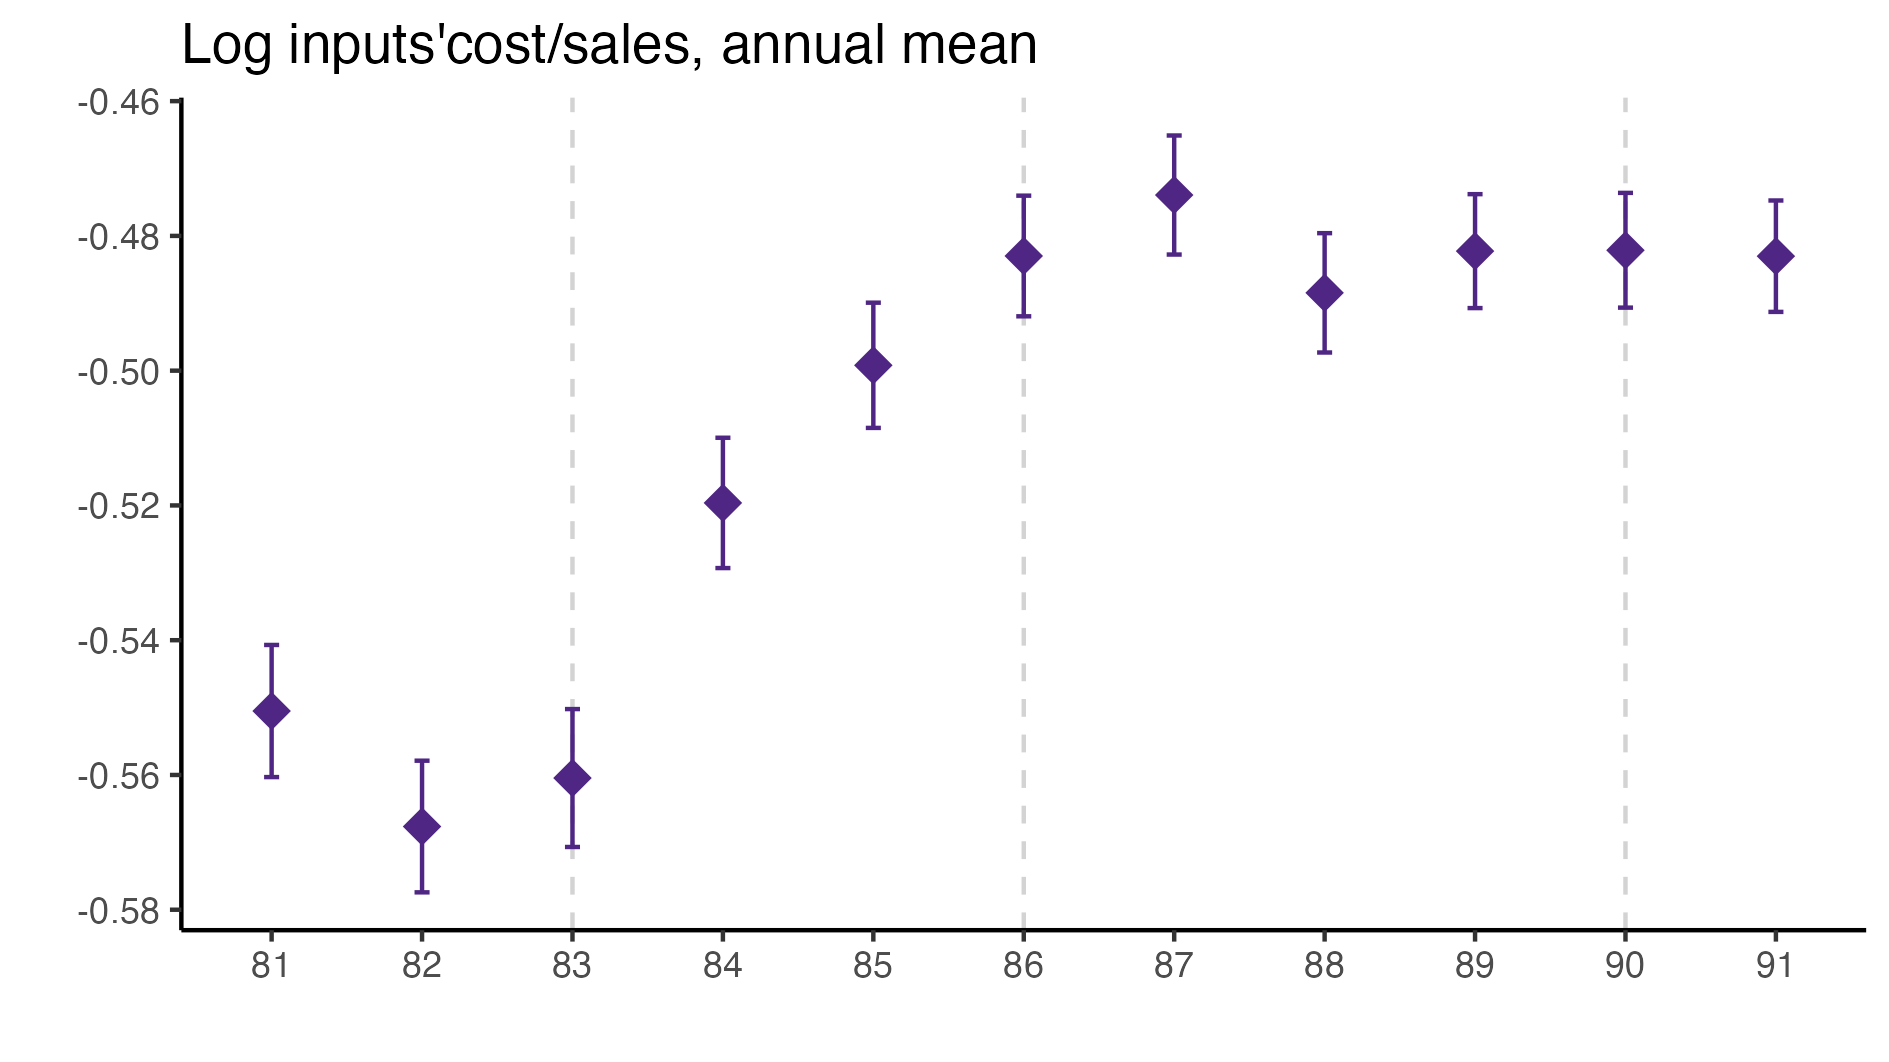
\includegraphics[width=1\textwidth,height=\textheight]{../Results/Figures/Colombia/log_share_byy.png}

}

\caption{\label{fig-logshare}Input's cost share of sales, average by
year of the logs.}

\end{figure}%

As a validation exercise, we can see that the VAT changes induced by the
three fiscal reforms are captured in the dataset. Figure~\ref{fig-vat}
shows that the sales tax increased to 10\% after the 1983 reform, and
then around 12\% after the 1990 reform.

\begin{figure}

\centering{

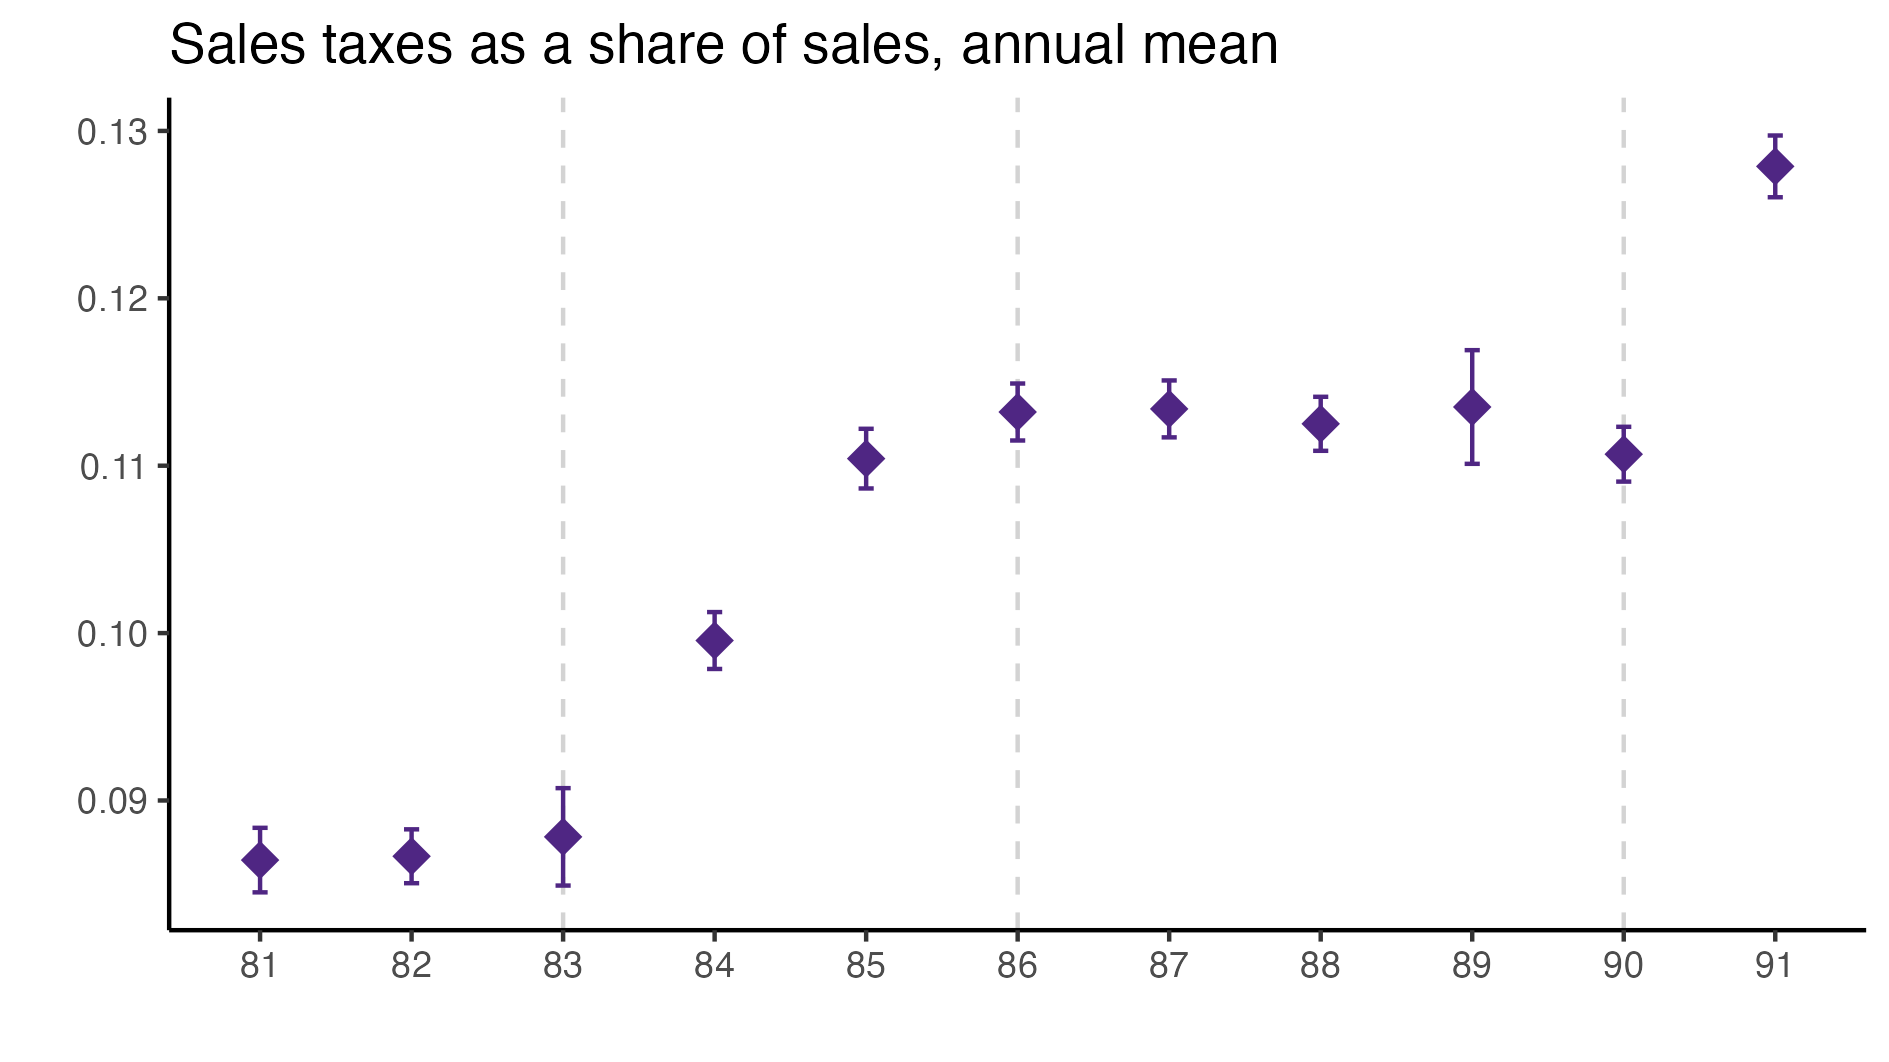
\includegraphics[width=1\textwidth,height=\textheight]{../Results/Figures/Colombia/share_sales_tax_byy.png}

}

\caption{\label{fig-vat}Sale taxes paid as share of sales, average by
year.}

\end{figure}%

Just as an exercise to see if other economic changes in this period were
driving the apparent changes in overreporting, Figure~\ref{fig-logsales}
shows that sales, for instance, were not exactly following the changes
in fiscal policy. Sales started to grow during 1983, the year of the
reform, whereas the cost share of sales started to grow the year after.
Likewise, sales fell in 1986, while the cost share seems to reduce its
growth after 1986.

\begin{figure}

\centering{

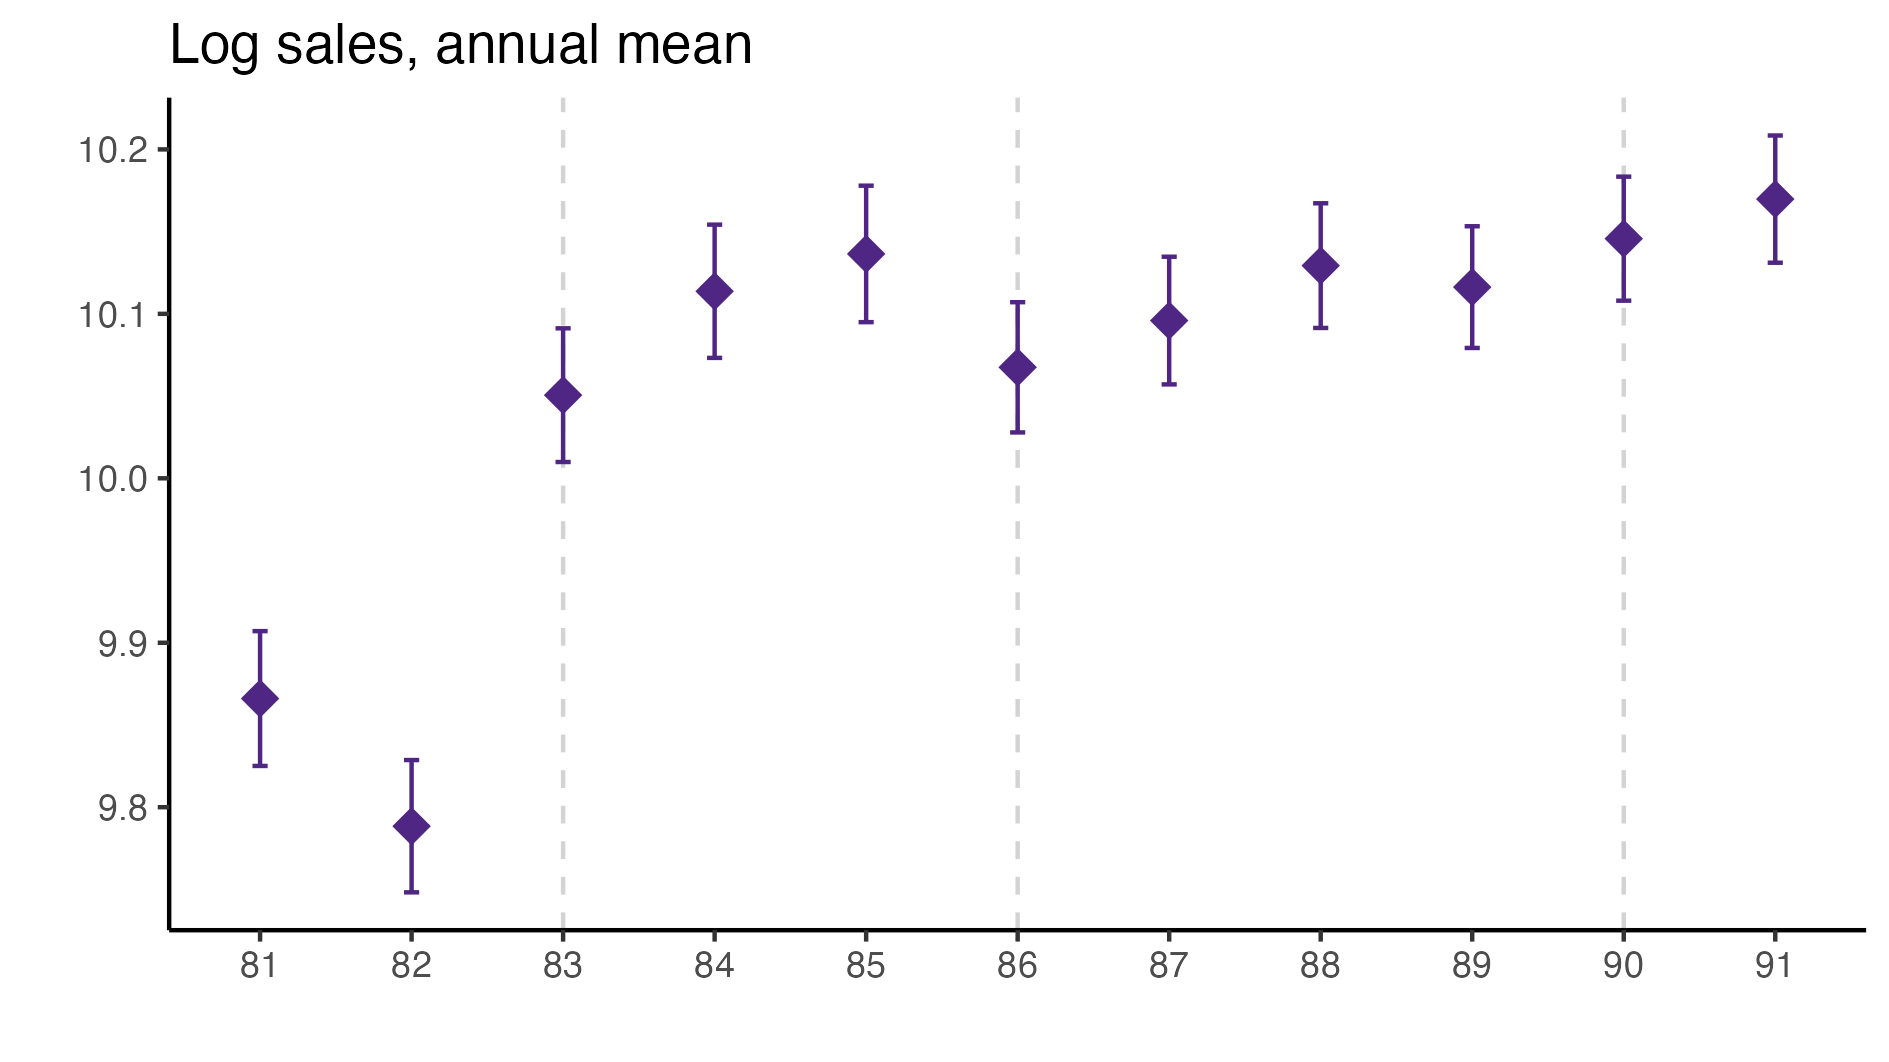
\includegraphics[width=1\textwidth,height=\textheight]{../Results/Figures/Colombia/log_sales_byy.png}

}

\caption{\label{fig-logsales}Sales in logs, annual mean.}

\end{figure}%

Finally, in a preliminary empirical assessment, I observe that the sales
tax rate is a significant determinant of the log share of revenue and
that non-corporations consistently use 13-17 percent more intermediates
than Corporations for a rich set of controls Table~\ref{tbl-reg-jo-tax}.
The results were estimated following Equation~\ref{eq-reg-tax-jo}

\begin{equation}\phantomsection\label{eq-reg-tax-jo}{
log(s_{it})= \alpha_1Tax_{it}+\mathbf{\beta}_1'JurOrg_i + \beta_2'JurOrg_i\times\gamma_t+ \gamma_t + \gamma_{ind} +\gamma_{metro} + \beta'Z+ \varepsilon_{it}
}\end{equation}

\begin{table}

\caption{\label{tbl-reg-jo-tax}Effect of the Juridical Organization Type
and Sales Tax on the Log Share of Intermediate Inputs.}

\begin{minipage}{\linewidth}

\begingroup
\centering
\begin{tabular}{lccc}
   \tabularnewline \midrule \midrule
   Dependent Variable: & \multicolumn{3}{c}{\(log(s)\)}\\
   Model:         & (1)            & (2)            & (3)\\  
   \midrule
   \emph{Variables}\\
   Sales Tax Rate & 0.2776$^{**}$  & 0.4019$^{***}$ & 0.3798$^{***}$\\   
                  & (0.1158)       & (0.0907)       & (0.0917)\\   
   Proprietorship & 0.1502$^{***}$ & 0.1236$^{***}$ & 0.1203$^{***}$\\   
                  & (0.0252)       & (0.0200)       & (0.0193)\\   
   Ltd. Co.       & 0.1647$^{***}$ & 0.1403$^{***}$ & 0.1352$^{***}$\\   
                  & (0.0265)       & (0.0210)       & (0.0210)\\   
   Partnership    & 0.1830$^{***}$ & 0.1588$^{***}$ & 0.1577$^{***}$\\   
                  & (0.0297)       & (0.0239)       & (0.0234)\\   
   \midrule
   \emph{Fixed-effects}\\
   Industry       &                & Yes            & Yes\\  
   Metro Area     &                &                & Yes\\  
   \midrule
   \emph{Fit statistics}\\
   Observations   & 41,830         & 41,830         & 41,830\\  
   R$^2$          & 0.54871        & 0.56214        & 0.56715\\  
   Within R$^2$   &                & 0.51571        & 0.51776\\  
   \midrule \midrule
   \multicolumn{4}{l}{\emph{Clustered (Industry \& Year) standard-errors in parentheses}}\\
   \multicolumn{4}{l}{\emph{Signif. Codes: ***: 0.01, **: 0.05, *: 0.1}}\\
\end{tabular}
\par\endgroup

\end{minipage}%

\end{table}%

Although this is not deterministic evidence, it does not contradict the
hypothesis that firms other than corporations have incentives to
overreport intermediates to evade taxes and that the higher the taxes
the higher the incentives to evade by misreporting.

\section{Identification Strategy}\label{identification-strategy}

Because the firms' optimization decisions depend on the fiscal
environment, the identification strategy should be motivated by the
fiscal environment \(\Gamma\). In particular, the identification
strategy will be as good as how well we can tell apart a subset of firms
that have the highest incentive to not evade. For example, in the case
of Spain, the firms above the revenue LTU threshold. In the case of
Colombia, the corporations.

\phantomsection\label{ass-non-ev}
\begin{fbx}{Assumption}{Assumption 4.1: }{Non-Evaders}
\phantomsection\label{ass-non-ev}
Based on the fiscal environment \(\Gamma\), the researcher can identify
a subset of firms \(\theta_i\in\Theta^{NE}\subset \Theta\) that does not
evade taxes by overreporting inputs.

\end{fbx}

For those firms, then \(\mathbb{E}[e_{it}|\theta_i\in\Theta^{NE}]=0\)

In addition, I impose the following timing assumption.

\phantomsection\label{ass-ind}
\begin{fbx}{Assumption}{Assumption 4.2: }{Independence}
\phantomsection\label{ass-ind}
Firms choose overreporting \(e_{it}\) \emph{before }the output shock
\(\varepsilon_{it}\)

\end{fbx}

Assumption \hyperref[ass-ind]{4.2} implies that input overreporting is
independent of the current period output shock,
\(e_{it} \perp \varepsilon_{it}\). In the literature is not rare to
assume that the output shock is not part of the information set of the
firms, \(\varepsilon_{it}\not\in \mathcal{I}_t\) \citep{Gandhi2020}.
Timing and information set assumptions are not uncommon for
identification strategies in production functions and demand estimation
\citep{Ackerberg2021, Ackerberg2019}.

\subsection{Identifying the production function
parameters}\label{identifying-the-production-function-parameters}

The econometrician observes then the overreported inputs in the data,
\(M_{it}=M^*_{it}\exp(e_{it})\)\footnote{Note we can always rewrite
  \(M^*+e=M^*\exp\{a\}\), then \(\exp\{a\}=\frac{e}{M^*}+1\).}. Assume
the production function is Cobb-Douglas,
\(G(M^*_{it}, K_{it}, L_{it})\exp(\omega_{it}+\varepsilon_{it})=M^{*\beta}_{it}K_{it}^{\alpha_K}L_{it}^{\alpha_L}\exp(\omega_{it}+\varepsilon_{it})\).
Then, for the case of Colombia, Equation~\ref{eq-foc:ind} applies since
the type of firms is the juridical organization and the non-evaders are
Corporations. By multiplying both sides by the intermediate inputs and
dividing by the output, we get

\begin{equation}\phantomsection\label{eq-foc-cd}{
\begin{aligned}
    \ln\left(\frac{\rho_t M^*_{it}}{P_{t}Y_{it}}\right)+e_{it}&=\ln\beta + \ln \mathcal{E}- \varepsilon_{it} \\
    &\equiv \ln D^{\mathcal{E}}- \varepsilon_{it} 
\end{aligned}
}\end{equation}

where,
\(\mathcal{E}\equiv \mathbb{E}[\exp(\varepsilon_{it})|\mathcal{I}_{it}]=\mathbb{E}[\exp(\varepsilon_{it})]\).

We can use Equation~\ref{eq-foc-cd} and assumption
\hyperref[ass-non-ev]{4.1} to recover the production function parameter
\(\beta\)

\begin{equation}\phantomsection\label{eq-foc-cd-exp}{
    \mathbb{E}\left[\ln\left(\frac{\rho_t M^*_{it}}{P_{t}Y_{it}}\right)\Bigg| \Theta^{NE}\right]=\ln D^{\mathcal{E}}
}\end{equation}

The constant \(\mathcal{E}\) is also identified \citep{Gandhi2020},

\begin{equation}\phantomsection\label{eq-id-E}{
\mathcal{E}=\mathbb{E}\left[\exp\left(\ln D^{\mathcal{E}}- \ln\left(\frac{\rho_t M^*_{it}}{P_{t}Y_{it}}\right)\right)|\theta^{NE}\right]=\mathbb{E}\left[\exp(\varepsilon_{it})|\theta^{NE}\right]=\mathbb{E}[\exp(\varepsilon_{it})]
}\end{equation}

and, thus, the output elasticity of input, \(\beta\), is also
identified,

\begin{equation}\phantomsection\label{eq-id-beta}{
\beta=\exp\left(\ln D^{\mathcal{E}}-\ln\mathcal{E}\right).
}\end{equation}

\subsection{Identifying Tax Evasion}\label{identifying-tax-evasion}

Having recovered both the flexible input elasticity, \(\beta\), and the
constant \(\mathcal{E}\), for all firms, I can form the following
variable using observed data.

\begin{equation}\phantomsection\label{eq-ob-ev}{
\begin{aligned}
    \mathcal V_{it}\equiv&\ln\left(\frac{\rho_t M_{it}}{P_{t}Y_{it}}\right)-\ln\beta -\ln\mathcal{E}\notag \\
    &=\ln\left(\frac{\rho_tM^*_{it}}{P_{t}Y_{it}}\right)-\ln\beta-\ln\mathcal{E}+e_{it} \notag \\
    &=-\varepsilon_{it} +e_{it}
\end{aligned}
}\end{equation}

By assumption \hyperref[ass-ind]{4.2}, the tax evasion,
\(\varepsilon_{it}\) ,is independent of \(e_{it}\). Note that, from
Equation~\ref{eq-foc-cd}, we also recovered
\(f_{\varepsilon}(\varepsilon)\) the distribution of \(\varepsilon\).
Tax evasion therefore can be recovered up to an independent random
variable by using deconvolution methods.

In particular, from probability theory,

\begin{definition}[]\protect\hypertarget{def-conv}{}\label{def-conv}

\begin{fbx}{Definition}{Definition: }{Convolution}
\phantomsection\label{}
The density of the sum of two \textbf{independent} random variables is
equal to the \textbf{convolution} of the densities of both addends;
hence

\[
h = f*m = \int f(\mathcal Z - \varepsilon)m(\varepsilon)d\varepsilon
\]

where \(f\) is the density of \(\mathcal Z\) (Meister, 2009)

\end{fbx}

\end{definition}

\subsection{Identifying Productivity}\label{identifying-productivity}

Here I show how to recover the rest of the parameters of the production
function, including productivity, and the Markov process of
productivity. We can do it in several ways, depending on our object of
interest.

In the literature, it is not uncommon to assume that productivity
follows a Markov process. That is,

\begin{equation}\phantomsection\label{eq-prod-markov}{
    \omega_{it}=h(\omega_{it-1})+\eta_{it}
}\end{equation}

We can form the following observed variable for a guess of
\(\alpha=(\alpha_K,\alpha_L)\),

\[
\begin{aligned}
    \mathcal W_{it}(\alpha) & \equiv \ln Y_{it} - \beta M_{it}-\alpha_K \ln K_{it}-\alpha_L \ln L_{it}+\beta\mathcal{V}_{it}\\
    & = \omega_{it}(\alpha)+(1-\beta)\varepsilon_{it}
\end{aligned}
\]

If we are interested only in productivity, we could use deconvolution to
learn \(\alpha\) and the distribution of productivity.

Alternatively, if we are interested in also identifying the Markov
process of productivity, we can use the orthogonality we get from
Equation~\ref{eq-prod-markov},
\(\mathbb{E}[\eta_{it}|k_{it},l_{it},k_{it-1},l_{it-1},\mathcal{W}_{it-1}]=0\).
Orthoganility follows from (\(k_{it-1},l_{it-1},\mathcal{W}_{it-1}\))
being known to the firm at period \(t-1\), and (\(k_{it-1},l_{it-1}\))
being predetermined.

Namely, substituting \(\omega_{it}\) in Equation~\ref{eq-prod-markov},
we have

\[
 \mathbb{E}[\mathcal{W}_{it}(\alpha)|k_{it},l_{it},,k_{it-1},l_{it-1},\mathcal{W}_{it-1}]=h(\mathcal{W}_{it-1}(\alpha))
\]

Thus, \(\alpha\) and \(h\) are identified.

\subsection{Translog Production
Function}\label{translog-production-function}

To relax the assumption of a CD production function, we would need a
flexible input that firms do not overreport to identify tax evasion.
Firms might face flexible inputs that they cannot deduct from their VAT
or CIT, for example. If this is the case, then firms would have no
incentives to overreport non-deductible flexible inputs.

Assume now that \(L_{it}\) is a non-deductible flexible input and,
without loss of generality, there are only two inputs
(\(L_{it}, M_{it}\)). Let's assume the production function is now
\emph{translog} and let \(\ln X_{it}=x_{it}\). We have,

\[
 \ln G(l,m)=\beta_0m_{it}+\beta_1m_{it}l_{it}+\beta_2m_{it}m_{it}+\beta_3l_{it}+\beta_4l_{it}l_{it}
\]

Then, equation Equation~\ref{eq-foc-cd} becomes

\[
\begin{aligned}
    s_{it}^{L}&=\ln \left(\beta_0+\beta_1l_{it}+\beta_2(m^*_{it}+e_{it})\right) + \ln \mathcal{E}- \varepsilon_{it} \\
    &\equiv \ln D^{\mathcal{E}}(l_{it},m^*_{it}+e_{it})- \varepsilon_{it} 
\end{aligned}
\]

where
\(s_{it}^{L} \equiv\ln\left(\frac{\rho^{L}_t L_{it}}{P_{t}Y_{it}}\right)\).

Note that by assumption \hyperref[ass-non-ev]{4.1}, \(D^{\mathcal{E}}\)
and the density of \(\varepsilon\) are still identified. To identify tax
evasion, we can form the analog of Equation~\ref{eq-ob-ev},

\[
\begin{aligned}
\mathcal{V}_{it}^{TL} &=\ln\left(\frac{\rho L}{PY}\right)-\ln D^{\mathcal{E}}(l,m^*+e)\\
    &=\ln\left(\frac{\rho L}{PY}\right)-\ln D^{\mathcal{E}}(l,m^*+e)\\
    &+\left[\ln D^{\mathcal{E}}(l,m^*)\right]\\
    &-\left[\ln D^{\mathcal{E}}(l,m^*)\right] \\
    &=\ln\left(\frac{\rho L}{PY}\right)-\ln D^{\mathcal{E}}(l,m^*) \\
    &-\left[\ln D^{\mathcal{E}}(l,m^*+e)-\ln D^{\mathcal{E}}(l,m^*)\right]\\
    &= -\varepsilon(l,m^*) - \delta(l,m^*,m^*+e)
\end{aligned}
\]

where in the case of the translog production function
\(\delta(l,m^*,m^*+e)\equiv \ln \left(\beta_0+\beta_1l_{it}+\beta_2(m^*_{it}+e_{it})\right)-\ln \left(\beta_0+\beta_1l_{it}+\beta_2m^*_{it}\right)\).
Note that is always positive \(\delta(l,m^*,m^*+e)\ge0\) because
\(e_{it}\ge0\).

Because firms cannot use \(l\) to deduct taxes, \(l\) is orthogonal to
\(e\). Hence, conditional on \(m^*\), \(\varepsilon(l,m^*)\) and
\(\delta(l,m^*,m^*+e)\) are independent. Thus, we can apply
deconvolution techniques again.

\subsection{Non-Parametric
Identification}\label{non-parametric-identification}

The previous result also suggests a non-parametric identification
strategy, as long as \(\delta(l,m^*,m^*+e)\) is monotonic in its
\(m^*+e\) argument. This identification strategy is analogous to
\citet{Hu2022b}, where the authors also require monotonicity and
independence to recover a nonparametric function of \(m^*\) with
nonclassical measurement error. In our case, intuitively, if we know the
density of \(\varepsilon\) and the function \(D^{\mathcal{E}}\), the
variation left is due to \(e\), which can be recovered as long as we can
vary \(\delta\) by moving \(e\).

To see why the non-deductible flexible input is needed to identify tax
evasion consider the following. Suppose that only the input \(M\) is
flexible and deductible.

\[
\ln\left(\frac{\rho M}{PY}\right)=\ln D^{\mathcal{E}}(K,L,M)-\varepsilon
\]

\(D^{\mathcal{E}}(K,L,M)\) is still identified by assumption
\hyperref[ass-non-ev]{4.1}, however, when we form the analogous of
Equation~\ref{eq-ob-ev}, we now have

\[
\begin{aligned}
\ln\left(\frac{\rho M}{PY}\right)-\ln D^{\mathcal{E}}(K,L,M)=&\ln\left(\frac{\rho(M^*+e)}{PY}\right)-\ln D^{\mathcal{E}}(K,L,M^*+e)\\
=&\ln\left(\frac{\rho(M^*+e)}{PY}\right)-\ln D^{\mathcal{E}}(K,L,M^*+e)\\
&+\left[\ln\left(\frac{\rho M^*}{PY}\right)-\ln D^{\mathcal{E}}(K,L,M^*)\right]\\
&-\left[\ln\left(\frac{\rho M^*}{PY}\right)-\ln D^{\mathcal{E}}(K,L,M^*)\right] \\
=&\ln\left(\frac{\rho M^*}{PY}\right)-\ln D^{\mathcal{E}}(K,L,M^*) \\
&+\left[\ln\left(\frac{\rho(M^*+e)}{PY}\right)-\ln\left(\frac{\rho(M^*)}{PY}\right)\right]\\
&-\left[\ln D^{\mathcal{E}}(K,L,M^*+e)-\ln D^{\mathcal{E}}(K,L,M^*)\right]\\
=& -\varepsilon \\
&+\left[\ln D^{\mathcal{E}}(K,L,M^*+e)-\varepsilon-\ln D^{\mathcal{E}}(K,L,M^*)+\varepsilon\right]\\
&-\left[\ln D^{\mathcal{E}}(K,L,M^*+e)-\ln D^{\mathcal{E}}(K,L,M^*)\right]\\
&= -\varepsilon(K,L,M^*)
\end{aligned}
\]

Now, we are not able to separate the variation of \(\varepsilon\) from
\(e\).

\section{Implementation}\label{implementation}

We are interested in the distribution of tax evasion \(e\) but it cannot
be observed. What is observed is the contaminated version
\(\mathcal{V}\) Equation~\ref{eq-ob-ev}. Evasion \(e\) and the output
shock \(\varepsilon\) are independent {[}\hyperref[ass-ind]{4.2}{]} with
probability density distributions \(f_e\) and \(f_{\varepsilon}\). Then,
from Definition~\ref{def-conv}

\[
f_{\mathcal{V}}(\mathcal{V})=\int f_{\varepsilon}(e-\mathcal{V})f_e(e)\text{d}e
\]

where \(f_{\mathcal{V}}\) denotes the density of \(\mathcal{V}\).

\subsection{Parametric MLE}\label{parametric-mle}

Assume a functional form for \(f_{\varepsilon}(\cdot;\gamma)\) that
depends on known parameters \(\gamma\). Assume a known functional form
for the density \(f_e(\cdot;\lambda)\) that depends on unknown
parameters \(\lambda\). We can estimate parameters \(\gamma, \lambda\)
by

\[
\arg \max_{\gamma,\lambda}=\frac{1}{n}\sum_{i=1}^n \log \left(\int f_{\varepsilon}(e-\mathcal{V};\gamma)f_e(e;\lambda)\text{d}e\right)
\]

Properties of MLE with unobserved scalar heterogeneity have been derived
elsewhere before \citep{Chen2007, Yi2021}.

\subsection{Non-Parametric MLE}\label{non-parametric-mle}

Consider the following log-density model:

\[
f_{e|\Theta}(e)=\exp(s(e;\theta)-C(\theta))
\]

where,

\[
s(e;\theta)=\sum_{j=1}^{k_n}\theta_j B_j(e),
\]

\(\{B_j(E), j=1,2,\dots\}\) is a sequence of known basis functions, and

\[
C(\theta) = \log\left(\int \exp(s(e;\theta)) \text{d}e \right)
\]

The log likelihood of the observed variable \(\mathcal{V}\) is

\[
\begin{aligned}
    l_{\mathcal{V}}(\mathbf{\theta})=&\sum_{i=1}^{n}\log \left(\int f_{\varepsilon}(e-\mathcal{V})\exp(s(e;\theta)-C(\theta))\text{d}e\right)\\
    =&\sum_{i=1}^{n}\log \left(\int f_{\varepsilon}(e-\mathcal{V})\exp(s(e;\theta))\text{d}e\right)-nC(\theta)
\end{aligned}
\]

The usual maximum likelihood estimate \(\hat{\theta}\) is the maximizer
of \(l_{\mathcal{V}}(\theta)\).

Laguerre polynomials can be used to approximate any function
\(L_2([0,\infty), leb)\) \(L_2\) norm relative to the Lebesgue measure
and domain \([0,\infty)\) \citep{Chen2007}.

The EM algorithm \citep{Kang2021} starts with an initial estimate
\(\hat{\mathbf{\theta}}^0\) and iteratively updates the estimate as
follows.

\textbf{Expectation-Step}: Given the current estimate
\(\hat{\mathbf{\theta}}^{(k)}\) of \(\hat{\mathbf{\theta}}\), calculate

\[
 b_j \left(\hat{\mathbf{\theta}}^{(k)}\right) = \sum_{i=1}^{n}\int B_j(e)f_{e|\mathcal{V},\hat{\theta}^{(k)}}(e|\mathcal{V})\text{d}e
\]

where,

\[
f_{e|\mathcal{V},\hat{\theta}}(e|\mathcal{V}) = f_{\varepsilon}(e-\mathcal{V})\exp(s(e;\theta)-C(\theta|\mathcal{V}))
\]

\[
C(\theta|\mathcal{V})=\log\left(\int f_{\varepsilon}(e-\mathcal{V})\exp(s(e;\theta))\text{d}e\right)
\]

\textbf{Maximization-Step}: Determine the updated estimate
\(\hat{\mathbf{\theta}}^{(k+1)}\) by maximizing

\[
Q(\mathbf{\theta}|\mathbf{\theta}^{(k)}) = \sum_{j=1}^{k_n}\theta_j b_j \left(\hat{\mathbf{\theta}}^{(k)}\right) - nC(\mathbf{\theta})
\]

The EM algorithm stops when
\(l_{\mathcal{V}}(\mathbf{\theta}^{(k+1)})-l_{\mathcal{V}}(\mathbf{\theta}^{(k)})<10^{-6}\).

\section*{References}\label{references}
\addcontentsline{toc}{section}{References}

\renewcommand{\bibsection}{}
\bibliography{biblio/export.bib,biblio/export2.bib,biblio/export3.bib,biblio/export31072022.bib,biblio/b100422.bib,biblio/b270123.bib,biblio/b100424.bib}




\end{document}
